\documentclass[12pt]{article}
\usepackage{amsmath,amssymb,amsthm}
\usepackage{graphicx,mathabx}
\usepackage{xcolor}
\usepackage{tikz}
\usepackage{placeins}
\usepackage{lipsum}
\usepackage[shortlabels]{enumitem}
\begin{document}
\title{TCSS 343 - Week 4}
\author{Jake McKenzie}
\maketitle
\noindent\centerline{\textbf{Dynamic Programming}}\\\\\\\\\\\\\\\\
\begin{center}
    ``An optimal policy has the property that whatever the initial state and initial decision are, the remaining decisions must constitute an optimal policy with regard to the state resulting from the first decision." \\$\cdots$\\  Richard Bellman's \textbf{Principle of Optimality}
\end{center}
\begin{center}
    ``What we choose means more than what was handed to us by chance." \\$\cdots$\\  Ada Palmer
\end{center}
\begin{center}
    `` If `dynamic programming' didn't have such a cool name, it would be known as 'populating a table'". \\$\cdots$\\ Mark Dominus 
\end{center}
\newpage
\noindent 1. Today we're going to explore dynamic programming. Below are three implementations of the fibonacci algorithm that I wrote in python. I want you to draw the \textbf{``tree"} for each then reflect on how the ``bottom up" apprach is different from the other two? (Hint: They are all trees but also different types of trees. This is a key insight in my opinion in idea in understanding dynamic programming) \\
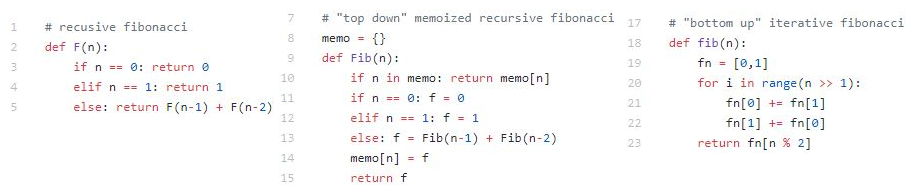
\includegraphics[width=\linewidth]{fib.jpg}
\newpage
\noindent 2. 
\end{document}